\section{Design Guidelines}
\label{sec:guidelines}

The following guidelines summarize the points discussed in the preceding sections as well as recommendations from other authors.
They serve as a basis for the design of head-up displays aiming to support the efficient completion of objectives without compromising safety.

To facilitate situation awareness, the HUD should be capable of providing as much information as possible without causing fatigue or sensory overload. The displayed information should be comprehensible in the shortest possible time. In an emergency, the system must be able to capture the user's attention without hindering decision-making or completely interrupting the primary task.

\subsection{Color and Contrast}

As mentioned in Section \ref{sec:AR}, the use of colors in HMDs intended for daylight use is primarily limited by current optical see-through technology. \textcite{gabbardPerceptualColorMatchingMethod2022} recommend to prefer colors with high source luminance, as these are less prone to color shifts. Furthermore, if a color typically represents a specific meaning and cannot be guaranteed to be perceived correctly, alternative colors that can meaningfully convey that message should be considered. Red is specifically cited as an example, as it is highly susceptible to color shifts due to its low luminance.

The library chroma.js\footnote{\href{https://gka.github.io/chroma.js/\#color-luminance}{chroma.js api docs!}} has a function to sort colors by luminance in the RGB color space, based on the Web Content Accessibility Guidelines 2.0.\footnote{\href{https://www.w3.org/TR/2008/REC-WCAG20-20081211/\#relativeluminancedef}{Web Content Accessibility Guidelines (WCAG) 2.0}} Sorting the base colors red (\#FF0000), green (\#00FF00), blue (\#0000FF) and their intermediaries cyan (\#00FFFF), magenta (\#FF00FF), and yellow (\#FFFF00) puts them into the following order (brightest to darkest): yellow, cyan, green, magenta, red, and blue.

\begin{figure}[hbt]
    \centering
    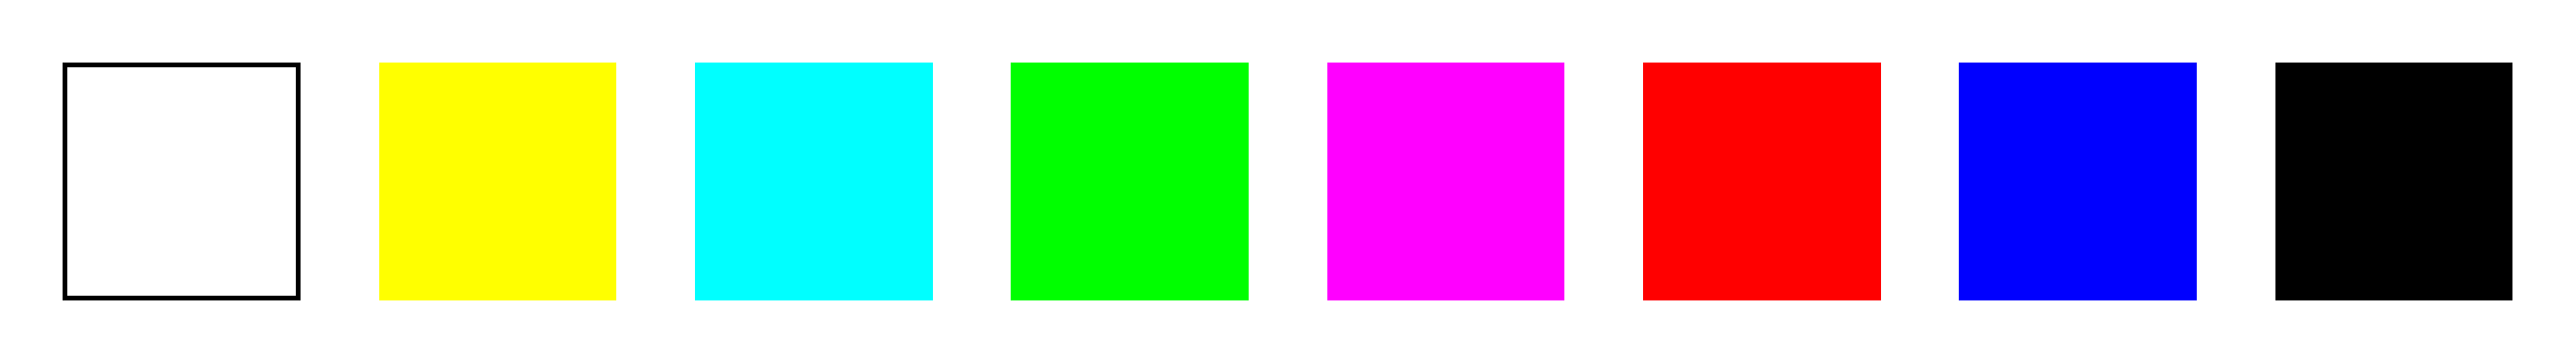
\includegraphics[width=1\textwidth]{assets/colors_luminance.eps}
    \captionbelow[Colors sorted by luminance]{Colors sorted by highest to lowest luminance, in order: yellow, cyan, green, magenta, red, and blue. White and black have been added for reference.}
    \label{fig:colors_sorted}
\end{figure}

Limiting the UI to a single color can ensure that the design functions effectively in every respect (e.g., by using motion to draw attention rather than color). Not encoding information through colors also avoids potential semantic misinterpretations that may be caused by the previously mentioned color issues.
In addition, monochrome displays are more affordable and therefore offer economic advantages, since replacement costs should be kept as low as possible in cases where equipment may be damaged or contaminated.

\subsection{Typography}

As with all head-mounted devices, walking causes them to shake, which affects legibility [\cite{janakaNotiFadeMinimizingOHMD2023}]. Especially thin, horizontal lines tend to disappear optically due to the up- and down motion.
\textcite{matsuuraReadabilityLegibilityFonts2019} confirm that heavier font weights improve readability. Naturally, the same requirements apply for stroke width in general.

For example, the typeface "Inter" meets these criteria well. It features a uniform stroke width, a square letter form and good line spacing. Compare this with the typeface "League Gothic", which also has a consistent stroke width, but due to its thickness, there is less white space within each character. Even with increased tracking, the narrowly shaped letters make reading considerably more difficult.

\begin{figure}[hbt]
    \centering
    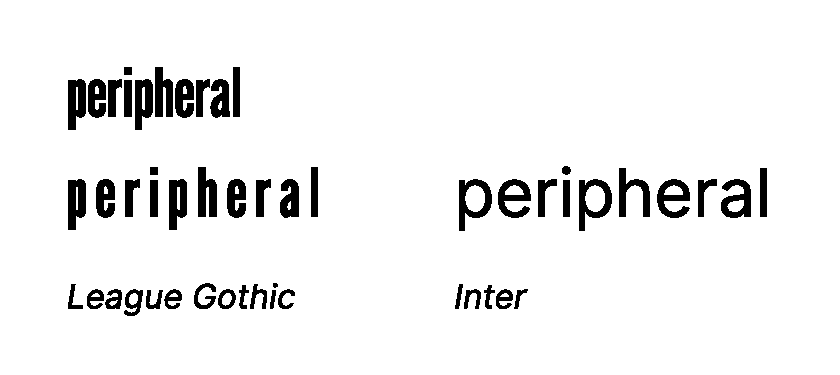
\includegraphics{assets/type_comparison.eps}
    \captionbelow[Legibility comparison of "Inter" and "League Gothic"]{A comparison of the legibility of the typefaces "Inter" and "League Gothic," both set at a size of 32 px and in the regular weight. For "League Gothic," a line with increased character spacing was added, demonstrating that the font remains difficult to read.}
    \label{fig:type_comparison}
\end{figure}

To determine optimal font sizes, \textcite{renkewitzOptimalFontSize2008} tested to what extent the background and font colors affect text recognition. They set a benchmark of two seconds as threshold for fast recognition, which resulted in recommended font sizes from 23 to 42 pt. However, these values may have to be adjusted for use on an OHMD, as they used a video see-through system and the colors red and blue, both of which have low luminance.

\textcite{gattulloLegibilityIndustrialAR2015} tested different text drawing styles in an indoor industrial setting. When the use of specific colors is mandated (e.g., in accordance with standard signage regulations), they recommend using white text on a billboard in the required color, which generally performed best. However, the billboard style obstructs much of the background. To remedy this, an outline style could be used, with thicker outlines further improving readability.

\begin{figure}[hbt]
    \centering
    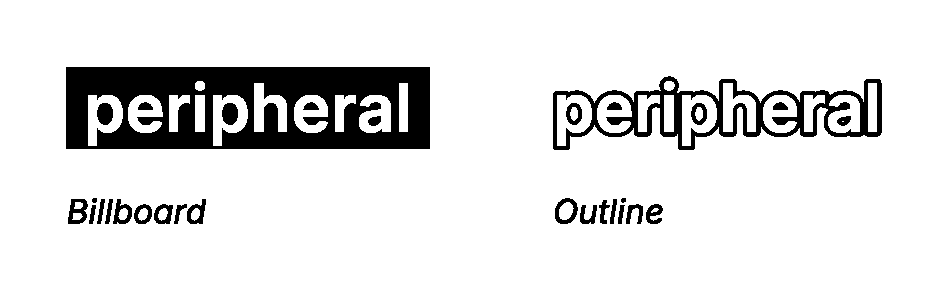
\includegraphics[width=0.9\textwidth]{assets/text_styles.eps}
    \captionbelow{Billboard and outline text drawing styles}
    \label{fig:text_styles}
\end{figure}

\subsection{Iconography}

\textcite{janakaCanIconsOutperform2023} tested if, and under which conditions icons perform better than text. They found that icon-augmented notifications enabled significantly higher primary task performance than text only and reduced the level of interruption while maintaining reaction and comprehension. They also found icons are more comprehensible when task complexity increased or demanded more attention. Additionally, the notification were "easier to perceive in suboptimal conditions", including outdoors when walking.

Naturally, this requires the icons to be easily recognizable. To that end, \textcite{linStudyRelationshipsDifferent2016} tested different versions of icons against each other. The differences tested were polarity, plane- and shape-based, and the presence or absence of borders. Since line-based icons dissect the space more frequently, they increase visual complexity, which impairs recognition performance. Overall, white shape-based icons on black background performed best.

\begin{figure}[hbt]
    \centering
    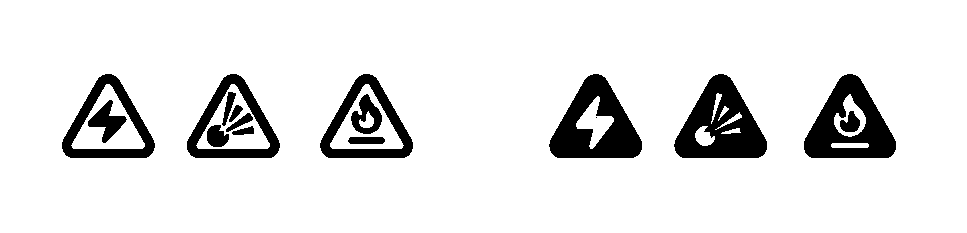
\includegraphics[width=0.9\textwidth]{assets/icons_line_shape.eps}
    \captionbelow{Line-based and plane-based icons}
    \label{fig:icons_hazard}
\end{figure}

\begin{figure}[hbt]
    \centering
    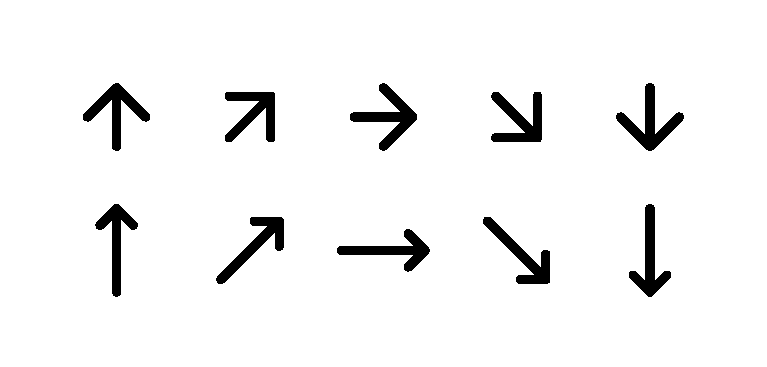
\includegraphics[width=0.8\textwidth]{assets/arrow_shape.eps}
    \captionbelow[Comparison of short and long arrows]{Comparison of short and long arrows.}
    \label{fig:arrow_shape}
\end{figure}

\textcite{lindbergEffectIconSpacing2003} point out that the size of icons has a greater impact on visual search performance than the spacing between them. However, a spacing of 0.5 to 1 symbol should be maintained. They additionally mention that a grid of 5 $\times$ 5 icons can be processed in one fixation.

\subsection{Layout and Spacing}

The ability of (binocular) head-mounted displays to display content anywhere within the field of view always presents a trade-off between immediate access to information and an unobstructed central line of sight. In use cases involving a great deal of physical activity, a clear field of view should of course be given greater priority.

\textcite{chuaPositioningGlassInvestigating2016} investigated the positioning of content on a monocular OST-HMD worn in front of the right eye. The display was divided into a 3 $\times$ 3 grid, spanning 12.5° vertically and 17° horizontally in both directions from the center.
The top and most peripheral positions were found to be more comfortable and unobtrusive, although middle and bottom center positions were perceived more quickly. The center-right was recommended as the best balance between both usability and comfort.
They mention that the ideal display position is highly dependent on task requirements (e.g., the center is preferable when driving, while secondary information is better placed in the periphery).

\textcite{linFindingOptimumPosition2021} divide HMD applications into four task categories: single (continuously focusing on display), alternating (switching back and forth between display and reality), background (passively monitoring the display for notifications) and dual (displayed information supplements physical primary task, e.g., live captions). Similar to \textcite{chuaPositioningGlassInvestigating2016}, they mention that optimal positioning depends on task type.
Participants preferred a horizontal angle of 5.4° to 14.6° and found angles beyond that to be uncomfortable.

\textcite{dowellEffectVisualLocation2002} mention 8° around the line of sight should be kept free, since it "can induce cognitive tunneling and impair performance on the task over which the HUD is superimposed." 
Ultimately, 8 to 20° horizontally seem to be a good compromise for most purposes [\cite{linFindingOptimumPosition2021}].

\subsection{Notifications}

Notification levels should be assigned according to the level of attention or action required. Each level should be coded as clearly as possible by choosing appropriate methods, such as abrupt movements for high urgency. If there are multiple independent high-priority notifications, they could be represented using different types of movement, such as flashing or bouncing. Furthermore, the more elements that attract attention, the less effective they are.

Although the billboard style occludes a large portion of the background around the text—which should generally be avoided—it is precisely this characteristic that makes it suitable for high-priority notifications.